\documentclass[letterpaper, 12pt]{article}
\usepackage{graphicx} % Required for inserting images
\usepackage{textcomp}
\usepackage{fullpage}
\usepackage{amsmath}
\usepackage{xcolor}
\usepackage{float}
\usepackage{enumitem}
\usepackage{geometry}
\geometry{margin=1in}
\usepackage{enumitem}
\usepackage{hyperref}
\usepackage{microtype}
\usepackage{gensymb}
\usepackage{parskip}
\usepackage{tikz}
\usepackage{pgfplots}
\pgfplotsset{compat=1.18}
\usepackage{nicefrac}
\hypersetup{
    colorlinks=true,        % Enable colored links
    linkcolor=teal,         % Set color for internal links
    citecolor=teal,         % Set color for citations
    filecolor=teal,         % Set color for file links
    urlcolor=teal           % Set color for URLs
}

\DeclareMathOperator{\arcsec}{arcsec}

\newcommand{\example}[1]{\textcolor{blue}{\textbf{Example:} #1}}
\newcommand{\step}[2]{\textcolor{blue}{\textbf{Step #1:} #2}}

\begin{document}

\begin{center}
\textbf{{\Large AP Calculus BC Test 5}}
\end{center}

\subsection*{H23 Parametric equations}

A parametric equation is a pair of equations that define a curve in the plane. The equations are typically written in the form $x = f(t)$ and $y = g(t)$, where $t$ is a \textbf{parameter} that varies over some interval.

The curve defined by the parametric equations can be traced out by varying the parameter $t$ from its starting value to its ending value, \underline{drawing arrows} to indicate directionality.

\subsubsection*{Eliminating the parameter}
To eliminate the parameter, solve one of the equations for $t$ and then substitute that expression into the other equation.

\example{Given the parametric equations $x = 2t + 1$ and $y = t^2 - 3$, eliminate the parameter to find an equation in terms of $x$ and $y$.}

\begin{gather*}
x = 2t + 1 \\
t = \frac{x - 1}{2} \\
y = t^2 - 3 \\
y = \left(\frac{x - 1}{2}\right)^2 - 3 \\
\boxed{y = \frac{(x - 1)^2}{4} - 3}
\end{gather*}

For trigonometric functions, use a Pythagorean identity.

\example{Given the parametric equations $x = 4\cos(t)$ and $y = 4\sin(t)$, eliminate the parameter to find an equation in terms of $x$ and $y$. Determine the shape of the curve.}

\begin{gather*}
x = 4\cos(t) \\
y = 4\sin(t) \\
\end{gather*}

Using the Pythagorean identity $\sin^2(t) + \cos^2(t) = 1$:

\begin{gather*}
\left(\frac{x}{4}\right)^2 + \left(\frac{y}{4}\right)^2 = 1 \\
\boxed{\frac{x^2}{16} + \frac{y^2}{16} = 1}
\end{gather*}

The curve is a \fbox{circle}.

\subsubsection*{Tangent lines}

$$\frac{dy}{dx} = \frac{\frac{dy}{dt}}{\frac{dx}{dt}}$$
$$\frac{d^2y}{dx^2} = \frac{\frac{d}{dt}\left(\frac{dy}{dx}\right)}{\frac{dx}{dt}}$$

\example{Find the slope of the tangent line to the curve and the concavity of the curve defined by the parametric equations $x = 4\cos(t)$ and $y = 4\sin(t)$ at the point where $t = \frac{\pi}{4}$.}

\step{1}{Find the first derivative and plug in the value of $t$ to get the slope.}

\begin{gather*}
\frac{dy}{dx} = \frac{\frac{dy}{dt}}{\frac{dx}{dt}} \\
= \frac{4\cos(t)}{-4\sin(t)} \\
= -\cot(t) \\
-\cot(t)|_{t = \frac{\pi}{4}} = -1 \\
\boxed{m = 1}
\end{gather*}

\step{2}{Find the second derivative and plug in the value of $t$ to get the concavity.}

Since we know $\frac{dy}{dx} = -\cot(t)$, differentiate and divide by $\frac{dx}{dt}$ to find the second derivative:

\begin{gather*}
\frac{d^2y}{dx^2} = \frac{\frac{d}{dt}\left(-\cot(t)\right)}{\frac{dx}{dt}} \\
= \frac{\csc^2(t)}{-4\sin(t)} \\
-\frac{\csc^2(t)}{4\sin(t)}|_{t = \frac{\pi}{4}} = -\frac{\sqrt{2}}{2} \\
\boxed{\text{concave down}}
\end{gather*}

\subsubsection*{Horizontal and vertical tangents}

If $\frac{dy}{dt} = 0$ and $\frac{dx}{dt} \neq 0$, then there is a \textbf{horizontal tangent}.

If $\frac{dx}{dt} = 0$ and $\frac{dy}{dt} \neq 0$, then there is a \textbf{vertical tangent}.

\subsubsection*{Arc length formula}

For parametric equations $x = f(t)$ and $y = g(t)$, the arc length from $t = a$ to $t = b$ is given by the formula:

$$L = \int_a^b \sqrt{\left(\frac{dx}{dt}\right)^2 + \left(\frac{dy}{dt}\right)^2} dt$$

\subsection*{H24 Vectors}

A vector is a quantity that has both magnitude and direction. Vectors can be represented in component form as $\mathbf{v} = \langle v_1, v_2 \rangle$.

\begin{description}
\item[position vector] $\mathbf{r}(t) = \langle x(t), y(t) \rangle$
\item [velocity vector] $\mathbf{v}(t) = \langle x'(t), y'(t) \rangle$
\item [acceleration vector] $\mathbf{a}(t) = \langle x''(t), y''(t) \rangle$
\end{description}

Below are the formulas for displacement, speed, and distance travelled:

\textbf{Displacement (vector), the change in position} (points from the starting position to the ending position)

$$\left \langle \int_{t_0}^{t_1} v_x(t) \, dt, \int_{t_0}^{t_1} v_y(t) \, dt \right \rangle$$

(note that \textbf{$v_x(t)$ and $v_y(t)$ are equivalent to $x'(t)$ and $y'(t)$}, respectively)

\textbf{Speed (scalar), the magnitude of the velocity vector}

$$\sqrt{v_x(t)^2 + v_y(t)^2}$$

or

$$\sqrt{x'(t)^2 + y'(t)^2}$$

\textbf{Distance travelled (scalar), the total length of the path taken}

Same as the arc length formula:

$$\int_{t_0}^{t_1} \sqrt{v_x(t)^2 + v_y(t)^2} \: dt$$

\example{An object moving along a curve in the $xy$-plane has position $(x(t), y(t))$ at time $t$ with $\frac{dy}{dt} = 2 + \sin\left(e^t\right)$. The derivative $\frac{dy}{dx}$ is not explicitly given. At $t=3$, the object is at the point $(4, 5)$. Find the $y$-coordinate of the position at time $t = 1$.}

\step{1}{Thinking logically, to find the $y$-coordinate at $t=1$, we work backwards from $t=3$ to $t=1$ using the given derivative $\frac{dy}{dt}$. $y(3)$ can be found by integrating $\frac{dy}{dt}$ from $t=1$ to $t=3$ and adding the result to $y(1)$, so to find $y(1)$, we can use the following formula:}

$$y(1) = 5 - \int_1^3 (2 + \sin(e^1)) \: dt$$

The change is being subtracted, not added, as we are going earlier in time.

Solving with a calculator, \boxed{y(1) \approx 1.27}

\subsection*{H25 Polar coordinates}

A polar coordinate is written in the form $(r, \theta)$, where $r$ is the distance from the origin and $\theta$ is the angle measured counterclockwise from the positive $x$-axis.

To convert polar to rectangular coordinates:

$$x = r\cos(\theta)$$
$$y = r\sin(\theta)$$

\subsubsection*{Area of a polar region}

The area of a region bounded by a polar curve $r = f(\theta)$ from $\theta = a$ to $\theta = b$ is given by the formula:

$$A = \frac{1}{2} \int_a^b (f(\theta))^2 \: d\theta$$

\example{Find the area bounded as shown by $r(\theta) = 2\cos(3\theta)$ and $r = \sqrt{3}$ with a calculator.}

\step{1}{Graph the equation.}

The area is the region between the two curves, which is shaded in the graph below:

\begin{figure}[H]
\centering
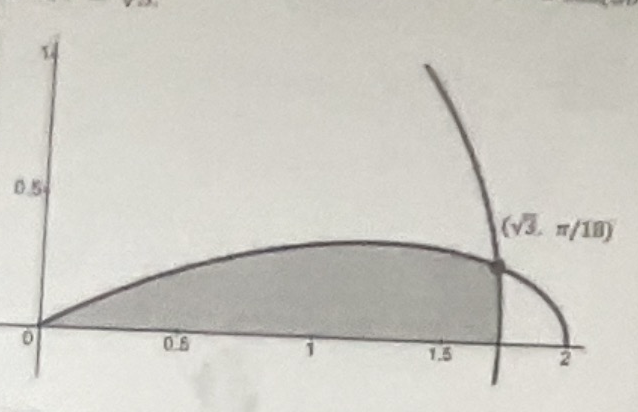
\includegraphics[width=0.5\textwidth]{petal.png}
\end{figure}

\step{2}{Find the points of intersection.}

The point of intersection $(\sqrt{3}, \frac{\pi}{18})$ is already given, but can be found by setting the two equations equal to each other ($2\cos(3\theta) = \sqrt{3}$) and solving for $\theta$.

\step{3}{Find where the bounds of the area are.}

The bounds of the area of the circle are $\theta = 0$ to $\theta = \frac{\pi}{18}$, and the bounds of the area of the petal are $\theta = 0$ to $\theta = \frac{\pi}{6}$ (found using a calculator).

\step{4}{Find the area.}

When integrating with respect to $\theta$, the bound is no longer the $x$-value or the $y$-value but the angle $\theta$. Essentially, we are finding the area underneath the function to the angle, not the area underneath the function to an axis.

Looking at the graph, the integral of the circle wrt $\theta$ can be added to the integral of the petal wrt $\theta$ from where the circle ends ($\frac{\pi}{18}$) to the end of the petal ($\frac{\pi}{6}$) to get the total area.

\begin{figure}[H]
\centering
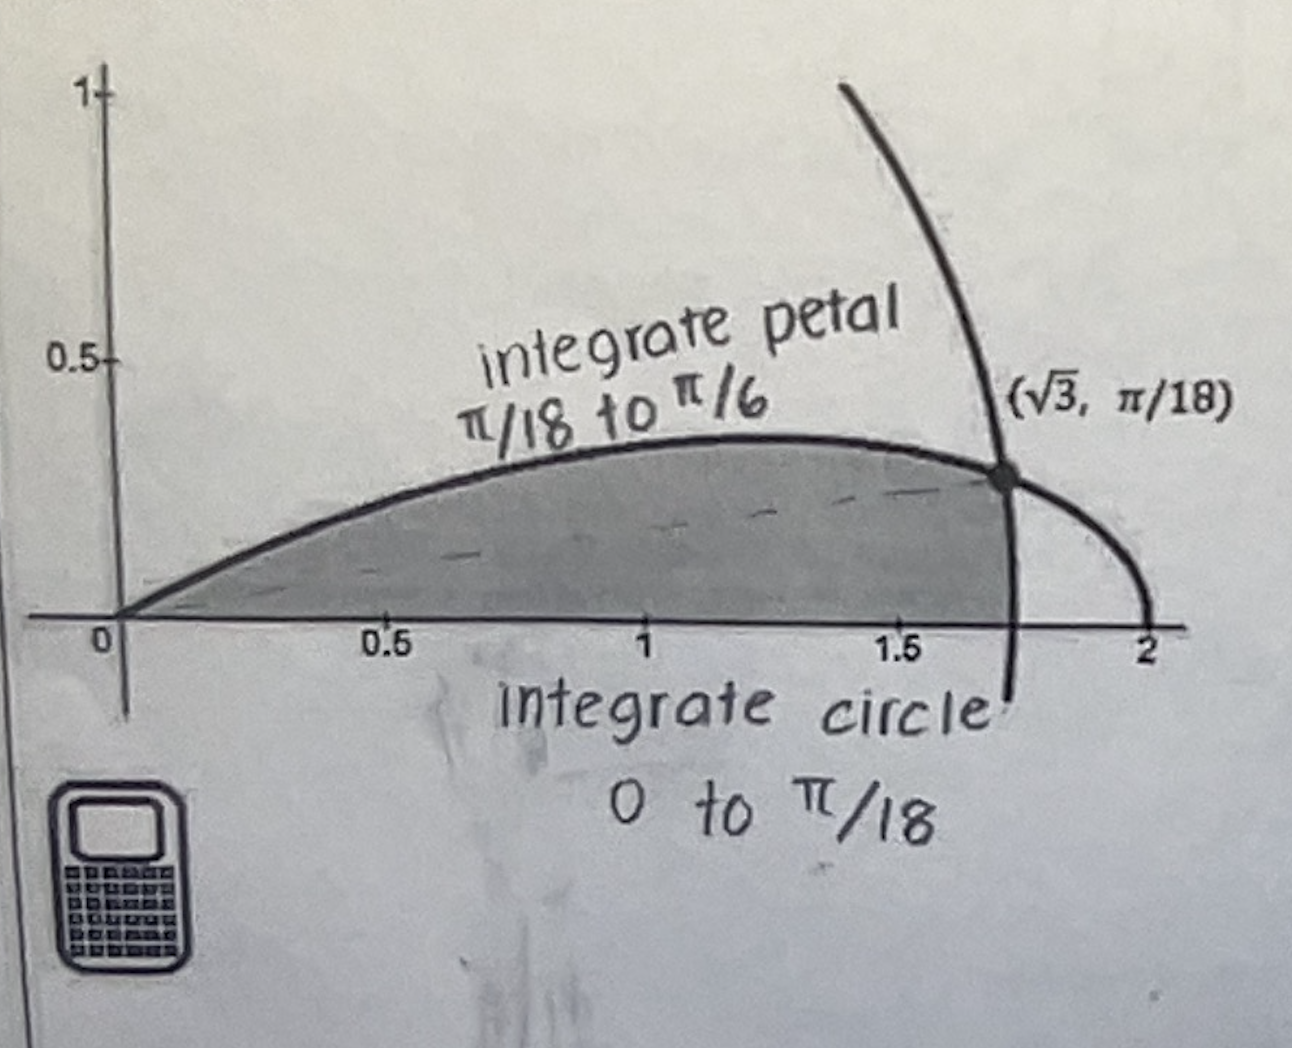
\includegraphics[width=0.5\textwidth]{petal2.png}
\end{figure}

First, the area of the circle that constitutes part of the petal:

$$A_{\text{circle}} = \frac{1}{2} \int_0^{\frac{\pi}{18}} (\sqrt{3})^2 \: d\theta$$

Now, the area remaining is calculated by taking the upper piece only (from $\pi/18$ to $\pi/6$):

$$A_{\text{petal}} = \frac{1}{2} \int_{\frac{\pi}{18}}^{\frac{\pi}{6}} (2\cos(3\theta))^2 \: d\theta$$

Using a calculator, computing

$$A = \frac{1}{2} \int_0^{\frac{\pi}{18}} (\sqrt{3})^2 + \: d\theta + \frac{1}{2} \int_{\frac{\pi}{18}}^{\frac{\pi}{6}} (2\cos(3\theta))^2 \: d\theta$$
$$\boxed{A \approx 0.467 \: \text{units}^2}$$

\example{Find the area between the outer loop and inner loop of $r = 2\theta\sin\theta$ for $\theta$ from $0$ to $2\pi$, inclusive.}

\step{1}{Graph the equation.}

\begin{figure}[H]
\centering
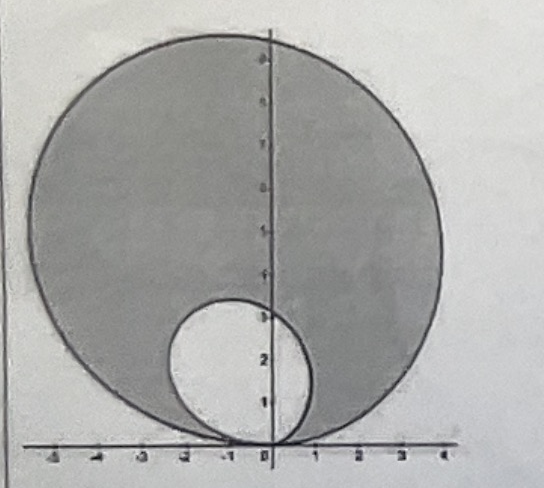
\includegraphics[width=0.5\textwidth]{loop_throwingmeforaloop.png}
\end{figure}

\step{2}{Find the bounds of the inner and outer loops with a calculator.}

Inner: $0 \leq \theta \leq \pi$ \\
Outer: $\pi \leq \theta \leq 2\pi$

\step{3}{Subtract the outer area from the inner area. Use a calculator to solve.}

\begin{gather*}
\int_0^{\pi} \frac{1}{2} (2\theta\sin\theta)^2 \: d\theta - \int_{\pi}^{2\pi} \frac{1}{2} (2\theta\sin\theta)^2 \: d\theta \\
= \boxed{62.013 \: \text{units}^2}
\end{gather*}

\end{document}